% CSE 598 Statistical Learning Theory -- Final Project Report
% Overleaf: Compiler = pdfLaTeX, bibliography via BibTeX.
\documentclass[11pt]{article}

\usepackage[margin=1in]{geometry}
\usepackage[T1]{fontenc}
\usepackage{lmodern}
\usepackage{amsmath,amssymb,amsthm}
\usepackage{mathtools}
\usepackage{graphicx}
\usepackage{booktabs}
\usepackage[font=small,skip=4pt]{caption}
\usepackage{subcaption}
\usepackage{xcolor}
\usepackage{enumitem}
\usepackage{algorithm}
\usepackage{algpseudocode}
\usepackage[numbers,sort&compress]{natbib}
\usepackage[colorlinks=true,linkcolor=blue!60!black,citecolor=blue!60!black,urlcolor=blue!60!black]{hyperref}
\usepackage[capitalize,noabbrev]{cleveref}

\graphicspath{{figures/}}

% ---- theorem environments (for stating the coverage guarantees) ----
\newtheorem{theorem}{Theorem}
\newtheorem{proposition}{Proposition}
\theoremstyle{definition}
\newtheorem{definition}{Definition}
\theoremstyle{remark}
\newtheorem{remark}{Remark}

% ---- notation shortcuts ----
\newcommand{\R}{\mathbb{R}}
\newcommand{\Prob}{\mathbb{P}}
\newcommand{\E}{\mathbb{E}}
\newcommand{\ind}[1]{\mathbf{1}\{#1\}}
\newcommand{\Qhat}{\widehat{Q}}
\newcommand{\yhat}{\hat{y}}

\title{Reliable Time-Series Anomaly Detection\\with Conformal Prediction and Foundation Models}
\author{
  Shreyanshi Dipinkumar Bhatt\\
  \small Arizona State University \quad \texttt{sbhat136@asu.edu}
  % Team project: list your partner as co-author if that is what the
  % instructor expects, e.g.  \and Ancy Pankajkumar Patel
}
\date{CSE 598: Statistical Learning Theory \\ Fall 2026}

\begin{document}
\maketitle

\begin{abstract}
Reliable anomaly detection in time series requires simultaneously identifying unusual behavior and controlling false alarms. Conformal prediction provides distribution-free finite-sample coverage guarantees under exchangeability, but time-series data violate this assumption through temporal dependence, distribution shift, and contamination of online calibration histories by anomalies themselves. We empirically study these effects using five one-step-ahead forecasters---including the zero-shot Chronos-Bolt foundation model---combined with four conformal thresholding strategies on five real-world series from the Numenta Anomaly Benchmark (NAB). At a target false-alarm rate of $\alpha=0.01$, split conformal produced approximately $1.56\%$ false alarms, whereas weighted conformal and Adaptive Conformal Inference (ACI) achieved rates near the target at $0.91\%$ and $0.94\%$, respectively. However, improved calibration did not imply improved anomaly detection: adaptive methods often incorporated anomalous observations into their updates and consequently widened their thresholds. To mitigate this effect, we introduce an episode-clipping variant of weighted conformal prediction that limits the influence of consecutive anomalous scores. It improved average detection F1 from $0.051$ to $0.071$ while retaining approximately $98.9\%$ normal-point coverage. Overall, our results reveal an important trade-off: adaptation can protect predictive coverage while simultaneously masking the anomalies a detector is intended to identify.
\end{abstract}

% =====================================================================
\section{Introduction}\label{sec:intro}

Time-series anomaly detection is important in applications such as industrial monitoring, cloud infrastructure, sensor networks, and transportation systems. In these settings, a monitoring system must identify unusual behavior quickly without generating an excessive number of false alarms. A natural strategy is to forecast the next observation and raise an alarm whenever the observed value differs substantially from the forecast. The central statistical problem is therefore not only producing an accurate forecast, but also determining how large a prediction error must be before it should be considered anomalous. A threshold that is too small produces frequent false alarms, whereas a threshold that is too large can conceal genuine failures.

Conformal prediction provides an attractive framework for constructing such thresholds. Given calibration data, conformal methods transform prediction errors into nonconformity scores and use their empirical distribution to construct prediction sets with a specified coverage level. Under exchangeability, classical conformal prediction provides finite-sample, distribution-free guarantees without requiring the forecasting model itself to be correctly specified \cite{vovk2005algorithmic,lei2018distribution,angelopoulos2023gentle}. Consequently, requesting $99\%$ coverage can be interpreted in anomaly detection as targeting approximately a $1\%$ false-alarm probability on normal observations.

The difficulty is that the standard exchangeability assumption is poorly matched to time-series data. Consecutive observations can be strongly dependent, the distribution can change between calibration and deployment, and anomalous observations can themselves enter an online method's calibration history. Several extensions have therefore been proposed. Adaptive Conformal Inference (ACI) adjusts its effective miscoverage level online \cite{gibbs2021adaptive}, while other approaches adapt conformal procedures to temporal or distributional changes \cite{zaffran2022adaptive}. Weighted conformal methods give greater importance to observations that are more representative of the current test point and provide bounds under nonexchangeability \cite{barber2023conformal}. Other theoretical work studies conformal inference directly under dependence and time-series assumptions \cite{chernozhukov2018exact,xu2021conformal,barber2026predictive}. Conformal ideas have also been applied specifically to anomaly detection \cite{laxhammar2015inductive,bates2023testing,martinezgil2026adaptive}.

At the same time, forecasting itself is changing rapidly. Time-series foundation models such as Chronos are pretrained on large collections of time series and can perform zero-shot forecasting on previously unseen datasets \cite{ansari2024chronos}. This raises an additional question for anomaly detection. A more accurate and adaptive forecaster should improve predictions on normal data, but an extremely adaptive model may also begin following an abnormal trajectory after a failure begins. Its prediction errors may then shrink precisely when persistent errors would be useful for detection.

This project studies the interaction between these two forms of adaptation---adaptation of the conformal threshold and adaptation of the forecasting model. We investigate four research questions:

\begin{enumerate}[leftmargin=*]
\item[\textbf{RQ1:}] Do nominal conformal coverage levels remain valid on real time series when exchangeability is violated?
\item[\textbf{RQ2:}] Does better conformal coverage necessarily lead to better anomaly detection?
\item[\textbf{RQ3:}] Does a zero-shot time-series foundation model improve anomaly detection compared with simpler forecasting models?
\item[\textbf{RQ4:}] For split conformal prediction, is loss of coverage more strongly associated with temporal dependence or distribution shift?
\end{enumerate}

We answer these questions through experiments on five real-world time series from the Numenta Anomaly Benchmark (NAB). Five forecasting configurations are evaluated: a naive persistence forecast, ARIMA, gradient boosting, Chronos-Bolt using its median prediction, and Chronos-Bolt using its predicted quantile interval. These forecasts are combined with split conformal, exponentially weighted conformal prediction, ACI, and a new episode-clipping modification of weighted conformal prediction.

Our experiments expose a distinction between \emph{coverage reliability} and \emph{anomaly-detection utility}. At $\alpha=0.01$, split conformal produces more false alarms than its nominal level, whereas weighted conformal and ACI achieve substantially better calibration. Nevertheless, split conformal has higher point-level anomaly recall and F1 in our experiments. The adaptive methods can absorb anomalous scores and increase their thresholds, causing them to stop alarming during persistent failures. A similar effect occurs at the forecasting level: Chronos can provide excellent zero-shot forecasts, yet its ability to adapt to a changing trajectory can make a failure less anomalous relative to its own prediction.

\paragraph{Contributions.}
\begin{itemize}[leftmargin=*,itemsep=2pt]
\item We provide an empirical comparison of five forecasting configurations and four conformal thresholding strategies on real, nonexchangeable time series, evaluating both statistical coverage and practical anomaly-detection performance.
\item We identify and analyze a coverage--detection trade-off: methods that adapt most effectively to maintain coverage can also adapt to anomalous episodes themselves, reducing detection recall. We show that an analogous phenomenon occurs for highly adaptive forecasting models.
\item We introduce an episode-clipping modification of weighted conformal prediction that limits contamination from consecutive anomalous scores. The method improves detection F1 over standard weighted conformal prediction at small $\alpha$ while retaining similar empirical coverage, although establishing a formal coverage guarantee remains future work.
\end{itemize}


% =====================================================================
\section{Problem Description}\label{sec:problem}

Consider a univariate time series $y_1, y_2, \ldots, y_T$ with $y_t \in \R$.
At time $t$, a one-step-ahead forecasting procedure observes only the history $\mathcal{F}_{t-1} = \{ y_1, \ldots, y_{t-1} \}$ and produces either a point prediction $\yhat_t$ or a predictive interval $[\ell_t, u_t]$. No future observations are available when the forecast is generated.

For a point forecaster, we define the nonconformity score as the absolute prediction error, $s_t = |y_t - \yhat_t|$. For a forecaster producing a base predictive interval, we instead use
\[
  s_t = \max\{ \ell_t - y_t,\; y_t - u_t,\; 0 \} .
\]
Thus, $s_t = 0$ when $y_t$ lies inside the base interval and increases according to the distance outside the interval. This is the score used for the Chronos quantile configuration following the conformalized quantile-regression principle \cite{romano2019conformalized}.

A conformal method constructs a threshold $q_t$ using previously observed nonconformity scores. We raise an alarm at time $t$ whenever $A_t = \ind{s_t > q_t} = 1$. The anomaly labels supplied by NAB are not used when generating test-time alarms. They are used only afterward to evaluate whether an alarm occurred during a known anomalous interval.

Let $z_t \in \{0, 1\}$ denote the ground-truth label, with $z_t = 0$ indicating a normal point and $z_t = 1$ an anomalous point. The objective is twofold: alarms should occur frequently enough during anomalous episodes to detect failures, while the alarm probability on normal observations should remain approximately below a user-selected level $\alpha$.

\begin{definition}[Coverage and false-alarm rate]\label{def:coverage}
Let $\mathcal{N} = \{ t \in \text{test} : z_t = 0 \}$ be the normal test points. The empirical coverage and false-alarm rate are
\[
  \widehat{\mathrm{Cov}} = \frac{1}{|\mathcal{N}|} \sum_{t \in \mathcal{N}} \ind{s_t \le q_t},
  \qquad
  \widehat{\mathrm{FAR}} = 1 - \widehat{\mathrm{Cov}} .
\]
A detector targeting miscoverage level $\alpha$ ideally satisfies
$\widehat{\mathrm{Cov}} \approx 1 - \alpha$, or equivalently
$\widehat{\mathrm{FAR}} \approx \alpha$.
\end{definition}

The basic motivation for using conformal prediction is that this relationship has a finite-sample justification under exchangeability.

\begin{theorem}[Split conformal coverage under exchangeability]\label{thm:split}
Let $s_1, \ldots, s_n, s_{n+1}$ be exchangeable nonconformity scores, where the first $n$ scores form the calibration sample. Define $k = \lceil (n+1)(1-\alpha) \rceil$ and let $q$ be the $k$-th smallest calibration score, with $q = +\infty$ if $k > n$. Then
\[
  \Prob(s_{n+1} \le q) \ge 1 - \alpha .
\]
Thus, the split-conformal prediction set has marginal coverage of at least $1-\alpha$ \cite{vovk2005algorithmic,lei2018distribution}.
\end{theorem}

\begin{proof}[Proof sketch]
Under exchangeability, the rank of $s_{n+1}$ among the $n+1$ scores is uniformly distributed over the possible ranks, up to ties. The event $s_{n+1} > q$ can occur only when the new score occupies one of the largest $(n+1) - k$ ranks. Therefore,
\[
  \Prob(s_{n+1} > q) \le \frac{n+1-k}{n+1} \le \alpha .
\]
Taking the complement gives $\Prob(s_{n+1} \le q) \ge 1 - \alpha$.
\end{proof}

This theorem illustrates the connection between conformal prediction and statistical learning theory: calibration observations are used to obtain a finite-sample guarantee on a future observation without imposing a parametric model for the score distribution. However, its symmetry argument depends critically on exchangeability.

Real time series violate this assumption in several ways. First, observations are temporally dependent. One formal characterization is $\beta$-mixing, under which dependence between events separated by $k$ time steps decreases as $k$ increases \cite{bradley2005basic}. Even when the marginal distribution is stationary, dependence reduces the amount of effectively independent calibration information. If $\tau_{\mathrm{int}}$ denotes an integrated autocorrelation time, a sample containing $n$ observations can behave approximately like only $n_{\mathrm{eff}} \approx n/\tau_{\mathrm{int}}$ independent observations.

Second, time series can undergo distribution shift. For example, temperature observations in one season need not have the same error distribution as observations several months later. A threshold estimated from calibration errors can therefore become systematically too small or too large in the test period.

Third, online conformal methods face \emph{contamination}. After an anomaly begins, the resulting large nonconformity scores are observed by the detector. If these scores are inserted directly into the calibration history, the detector can adapt its own threshold to the failure. The anomaly then becomes part of the distribution against which subsequent anomalous observations are compared.


% =====================================================================

\section{Methodology}\label{sec:method}

\subsection{Data}

We evaluate the methods using five time series from the \emph{realKnownCause} category of the Numenta Anomaly Benchmark (NAB) \cite{lavin2015evaluating,ahmad2017unsupervised}. This category contains real-world signals with labeled anomaly windows for which the causes of abnormal behavior are known. The selected datasets represent heterogeneous domains and sampling frequencies: office temperature, server CPU utilization, cloud-server latency, industrial machine temperature, and New York City taxi demand. Their sizes range from $4{,}032$ to $22{,}695$ observations.

Each series is divided chronologically into $40\%$ training, $15\%$ calibration, and $45\%$ testing data, as summarized in \cref{tab:datasets}. Chronological splitting is essential because randomly shuffling a time series would allow future observations to influence models intended to operate online.

The training partition is used only by forecasting models that require fitting. We do not remove anomalous observations from the training data because such information would generally be unavailable when training a detector in practice. For conformal calibration, however, labeled anomaly points are removed from the calibration partition. This represents a clean-calibration assumption: the initial reference scores are assumed to represent normal behavior, consistent with the motivation of conformal anomaly-detection procedures such as \cite{bates2023testing}. The test set is not cleaned and contains all labeled anomalous episodes. Labels are hidden from the forecasting and conformal procedures during prediction and are used only to calculate evaluation metrics.

\begin{table}[t]
\centering\small
\caption{The five NAB \emph{realKnownCause} series. Splits are chronological:
$40\%$ train, $15\%$ calibration, $45\%$ test.}
\label{tab:datasets}
\begin{tabular}{lccccc}
\toprule
Series & Length & Sampling & Windows & Windows in test & Anomalous points \\
\midrule
\texttt{ambient\_temp} & 7,267 & 60 min & 2 & 1 & 10.0\% \\
\texttt{cpu\_asg} & 18,050 & 5 min & 1 & 1 & 8.3\% \\
\texttt{ec2\_latency} & 4,032 & 5 min & 3 & 2 & 8.6\% \\
\texttt{machine\_temp} & 22,695 & 5 min & 4 & 2 & 10.0\% \\
\texttt{nyc\_taxi} & 10,320 & 30 min & 5 & 5 & 10.0\% \\
\bottomrule
\end{tabular}

\end{table}

\subsection{Forecasters}

We compare five forecasting configurations ranging from a simple persistence baseline to a pretrained foundation model. All forecasts are strictly one step ahead: the prediction at time $t$ uses only information available before $y_t$ is observed.

\paragraph{Naive persistence.}
The naive model predicts $\yhat_t = y_{t-1}$. It requires no fitting and provides an important baseline because many high-frequency sensor signals change gradually.

\paragraph{ARIMA.}
We fit an ARIMA$(2,1,2)$ model on the training partition \cite{box2015time}. Its parameters are estimated from training data and then held fixed during evaluation, while the latent state is updated sequentially through the model's filtering procedure. This provides a classical statistical time-series baseline.

\paragraph{Gradient boosting.}
The gradient-boosting model uses the previous 24 observations as lagged features together with rolling summary statistics, including the recent mean and standard deviation. Gradient-boosted regression trees combine multiple weak regression trees to model nonlinear relationships \cite{friedman2001greedy}. The implementation uses standard machine-learning utilities from scikit-learn \cite{pedregosa2011scikit}. The model is trained only on the training partition and is not refit during the test period.

\paragraph{Chronos-Bolt.}
Chronos is a pretrained time-series foundation model designed to perform forecasting across heterogeneous series \cite{ansari2024chronos}. We use Chronos-Bolt-small in a zero-shot setting, meaning that no parameters are fitted to any of the five NAB series. At each time step, the model receives up to the previous 512 observations as context and predicts the next observation. For the point-forecast configuration, the median forecast is used as $\yhat_t$.

\paragraph{Chronos-CQR.}
The second Chronos configuration uses the model's $0.1$ and $0.9$ predictive quantiles to obtain a base interval $[\ell_t, u_t]$. We then conformalize this interval using the score
\[
  s_t = \max\{ \ell_t - y_t,\; y_t - u_t,\; 0 \},
\]
following the conformalized quantile-regression construction of \cite{romano2019conformalized}. This configuration allows us to test whether information about predictive uncertainty from the foundation model improves anomaly detection relative to conformalizing only its median forecast.

\subsection{Conformal Thresholding Methods}

All methods receive a sequence of nonconformity scores and determine a threshold $q_t$ such that an alarm is produced whenever $s_t > q_t$.

\paragraph{Split conformal.}
The split method computes a single threshold from the clean calibration scores. If there are $n$ calibration observations, the threshold is the $\lceil (n+1)(1-\alpha) \rceil$-th order statistic. This threshold remains fixed throughout testing. Under exchangeability, \cref{thm:split} provides marginal coverage of at least $1-\alpha$. Its primary limitation in this setting is its inability to react to distribution shift.

\paragraph{Exponentially weighted conformal.}
The weighted procedure assigns greater importance to recent scores. A score observed $k$ steps in the past receives weight proportional to $w_k = \rho^k$, where the main experiments use $\rho = 0.999$. The threshold is computed as a weighted $(1-\alpha)$ quantile, including the appropriate mass at $+\infty$ in the nonexchangeable conformal construction \cite{barber2023conformal}. Exponential weighting gives the method an effective memory on the order of $1/(1-\rho)$. This allows it to react to changing score distributions, but also makes recent anomalous observations influential.

\paragraph{Adaptive conformal inference (ACI).}
ACI \cite{gibbs2021adaptive} replaces the fixed level $\alpha$ with a running level $\alpha_t$, computes $q_t$ as the conformal $(1-\alpha_t)$ quantile of recent scores, and updates
\[
  \alpha_{t+1} = \alpha_t + \gamma(\alpha - \mathrm{err}_t),
  \qquad \mathrm{err}_t = \ind{s_t > q_t},
\]
where $\gamma = 0.005$ in our primary experiments. If an observation is covered, $\alpha_t$ increases slightly; if it is not covered, $\alpha_t$ decreases. This feedback mechanism controls long-run average miscoverage under extremely weak assumptions. In anomaly detection, however, an anomalous observation is intentionally expected to violate the interval. ACI nevertheless treats this exceedance as an error requiring compensation, which can rapidly widen subsequent intervals.

For example, with $\alpha = 0.01$ and $\gamma = 0.005$, one exceedance changes $\alpha_t$ by $0.005(0.01 - 1) = -0.00495$. Starting from $0.01$, only a few consecutive alarms are therefore sufficient to drive the effective level to its boundary, producing an extremely conservative threshold. This explains why ACI can maintain excellent long-run coverage while temporarily becoming insensitive during an anomalous episode.

\paragraph{Weighted conformal with episode clipping.}
To reduce contamination of the weighted history, we introduce an episode-clipping variant. The procedure is identical to weighted conformal prediction except when alarms occur consecutively. The first alarm in a possible episode is stored normally. If the next observation is also flagged, its score is capped at a value immediately above the current threshold before being inserted into the weighted history. Further consecutive flagged scores are treated similarly.

The intuition is that an isolated exceedance can plausibly be a normal false alarm and should therefore remain untouched. By contrast, persistent anomalies often produce runs of very large scores. Without clipping, these recent high-weight scores can rapidly increase the weighted quantile and cause the detector to adapt to the anomaly.

For independent normal observations whose alarm probability is approximately $\alpha$, two consecutive false alarms occur with probability approximately $\alpha^2$. At $\alpha = 0.01$, this is $10^{-4}$, so episode clipping should rarely modify ordinary observations under this idealized approximation. This is an intuition rather than a formal coverage guarantee, particularly because real time-series alarms are dependent.

We also evaluated an earlier design that clipped every flagged observation. That version produced a threshold ratchet: once scores above the threshold were repeatedly capped, the history contained insufficient information to allow the threshold to move upward naturally. On an i.i.d.\ sanity check, the method produced approximately $1.66\%$ false alarms at a $1\%$ target. Restricting clipping to consecutive alarms removed this failure mode in the small-$\alpha$ regime.

\begin{algorithm}[t]
\caption{Online weighted conformal thresholding with episode clipping (ours)}
\label{alg:clip}
\begin{algorithmic}[1]
\Require calibration-score history $\mathcal{H}$, level $\alpha$, decay $\rho$, maximum history window $W$
\State $\mathrm{prevAlarm} \gets \mathrm{false}$
\For{$t = 1, 2, \ldots$}
  \State Assign exponentially decaying weights $w_i = \rho^{\,t-i}$ to scores in $\mathcal{H}$
  \State Compute the weighted $(1-\alpha)$ conformal quantile $q_t$
  \State Obtain the one-step forecast and observe $y_t$
  \State Compute nonconformity score $s_t$
  \State $A_t \gets \ind{s_t > q_t}$
  \If{$A_t = 1$ \textbf{and} $\mathrm{prevAlarm} = \mathrm{true}$}
    \State $\widetilde{s}_t \gets q_t^{+}$ \Comment{cap inside an alarm episode}
  \Else
    \State $\widetilde{s}_t \gets s_t$
  \EndIf
  \State Append $\widetilde{s}_t$ to $\mathcal{H}$ and retain at most the most recent $W$ scores
  \State $\mathrm{prevAlarm} \gets (A_t = 1)$
\EndFor
\end{algorithmic}
\end{algorithm}

\subsection{Evaluation Protocol}

The main experiment evaluates the Cartesian product of five datasets, five forecasting configurations, and four conformal methods at $\alpha = 0.01$. Performance is assessed from both a calibration perspective and a detection perspective.

For calibration, we report coverage on normal test observations, the corresponding miscoverage rate, false alarms per day, and interval width where applicable. For anomaly detection, we report point-level precision, recall, and F1 score. Because NAB labels failures as windows rather than isolated points, we additionally report the number of anomaly windows containing at least one alarm and the detection delay from the beginning of an anomalous window to its first alarm. The event-level metrics are important because point recall can appear artificially low when a labeled window is much wider than the portion of the failure that is statistically unusual.

Five groups of experiments are performed. \textbf{E1} is the main comparison at $\alpha = 0.01$. \textbf{E2} sweeps $\alpha$ from $0.005$ through $0.2$ to test whether empirical miscoverage tracks the nominal level. \textbf{E3} varies ACI's step size $\gamma$ and the weighted method's decay parameter $\rho$ to evaluate sensitivity to adaptation speed. \textbf{E4} investigates why split-conformal coverage fails by comparing its coverage gap with measures of distribution shift and temporal dependence. Finally, \textbf{E5} applies the conformal procedures to simulated i.i.d.\ data as a correctness check; methods derived under exchangeability should approximately recover their target miscoverage in this controlled setting.

Distribution shift is quantified using the Kolmogorov--Smirnov (KS) distance between the calibration-score and test-score distributions. Temporal dependence is summarized through an effective sample-size approximation $n_{\mathrm{eff}} = n/\tau_{\mathrm{int}}$, where $\tau_{\mathrm{int}}$ is the integrated autocorrelation time. A small effective sample size indicates that dependence makes the calibration set contain substantially less independent information than its nominal number of observations suggests.

Experiments were executed on CPU. Statistical time-series functionality was implemented using statsmodels \cite{seabold2010statsmodels}, and the gradient-boosting pipeline used scikit-learn \cite{pedregosa2011scikit}. The complete experimental pipeline was implemented chronologically to prevent test-to-train leakage.

% =====================================================================
\section{Results}\label{sec:results}

\subsection{Does coverage hold? (RQ1)}

The first result is that classical split-conformal coverage does not transfer perfectly to these time-series data. At the primary target $\alpha = 0.01$, split conformal produces a median of approximately $1.56\%$ false alarms on normal observations rather than the requested $1\%$. Across the smaller values of $\alpha$ in the sweep, its empirical miscoverage is approximately $1.5$--$1.7$ times the nominal level. Thus, the exchangeable finite-sample guarantee in \cref{thm:split} should not be interpreted as an unconditional guarantee for these temporally ordered data.

In contrast, the adaptive procedures track the target substantially more closely. At $\alpha = 0.01$, weighted conformal gives approximately $0.91\%$ normal-point miscoverage and ACI approximately $0.94\%$. This result supports the motivation for using online or nonexchangeable conformal methods when the score distribution changes over time.

The i.i.d.\ sanity experiment provides an important control. On simulated exchangeable data, the methods recover approximately the requested miscoverage. Therefore, the excess false-alarm rate observed for split conformal on NAB is unlikely to be simply an implementation artifact. Instead, it is consistent with violations of the assumptions connecting calibration scores to future test scores.

\cref{fig:calibration} shows this effect across the $\alpha$ sweep. A perfectly calibrated method would lie near the diagonal $y = \alpha$. Deviations above this line correspond to excessive false alarms, while deviations below it correspond to conservative thresholds. The gap for split conformal is most important operationally at small $\alpha$, where even a seemingly small absolute calibration error can represent a large relative increase in false alarms.

\begin{figure}[t]
\centering
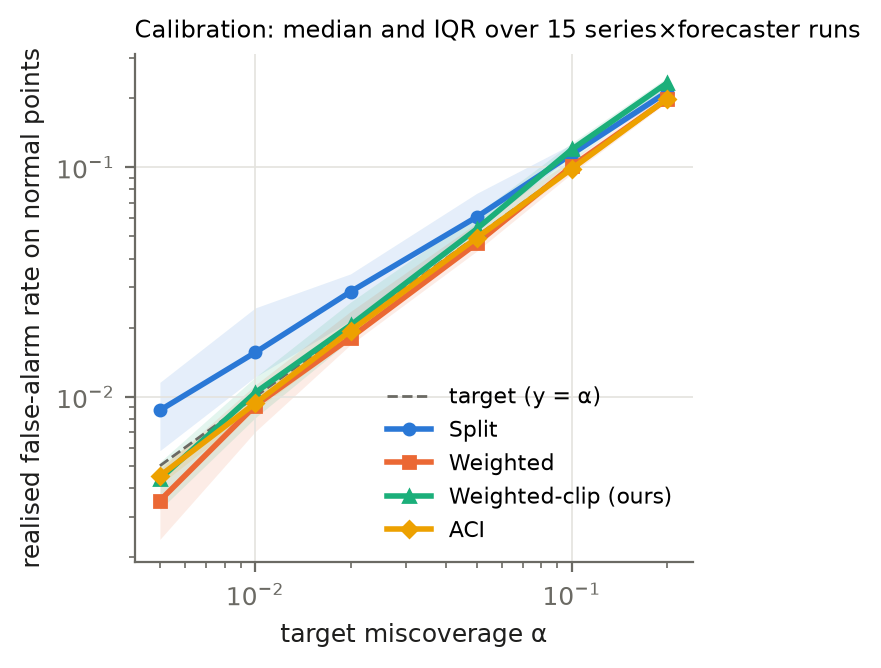
\includegraphics[width=0.42\linewidth]{fig_alpha_calibration.png}
\caption{Realized false-alarm rate on normal test observations versus the target
miscoverage level $\alpha$ on logarithmic axes. Lines show the median across
the evaluated series--forecaster combinations and shaded bands show the
interquartile range. The dashed diagonal represents perfect calibration,
$\widehat{\mathrm{FAR}} = \alpha$. Values above the diagonal indicate
anti-conservative behavior.}
\label{fig:calibration}
\end{figure}

\subsection{Does coverage imply detection? (RQ2)}

The central empirical finding is that improved coverage does \emph{not} imply improved anomaly detection. At $\alpha = 0.01$, split conformal has approximately $98.2\%$ normal-point coverage, below the nominal $99\%$, but obtains point recall $0.070$ and F1 $0.109$. Weighted conformal improves coverage to approximately $99.1\%$, yet recall falls to $0.028$ and F1 to $0.051$. ACI also achieves approximately $99.1\%$ coverage but has recall only $0.015$ and F1 $0.029$. Episode clipping lies between these extremes, with approximately $98.9\%$ coverage, recall $0.042$, and F1 $0.071$.

Detection delay follows the same pattern. The average reported delay is approximately $18.6$ hours for split conformal, compared with $22.4$ hours for weighted conformal, $21.5$ hours for weighted-clip, and $25.9$ hours for ACI. Therefore, the methods that most closely enforce the nominal false-alarm rate are not necessarily those that identify abnormal behavior fastest.

This apparent contradiction is explained by the role of adaptation. Suppose a persistent failure causes several unusually large scores. A static split threshold does not react: every sufficiently large subsequent score continues to exceed the same $q$. Weighted conformal instead inserts the anomalous scores into its recent history. Because recent scores receive the largest weights, the weighted upper quantile increases. The detector can consequently begin treating the failure as part of its new reference distribution.

ACI reacts even more directly: as computed in \cref{sec:method}, a short sequence of alarms pushes $\alpha_t$ to its boundary. The resulting prediction set becomes extremely wide, and the detector temporarily stops alarming. From ACI's calibration perspective this behavior is sensible: repeated exceedances indicate that the current intervals are too narrow. From an anomaly-detection perspective, however, those exceedances are precisely the observations that the system should continue identifying.

\cref{fig:intervals} illustrates this mechanism visually. During an anomalous episode, the adaptive intervals can expand after the first alarms, reducing subsequent exceedances. \cref{fig:tradeoff} confirms that the phenomenon is not limited to a single operating point: varying $\alpha$ produces a systematic trade-off between false alarms and recall.

Point-level recall alone, however, understates practical event detection on NAB because its anomaly windows can contain many observations. Across the experiment, the conformal methods raise at least one alarm in approximately $49$--$51$ of the $55$ evaluated anomaly windows, even though point recall ranges only from approximately $0.015$ to $0.070$. Thus, low point-level F1 should not be interpreted as meaning that almost all failure episodes are missed. Rather, adaptive methods tend to alarm near part of an episode and then adapt to its continuation.

\begin{figure}[t]
\centering
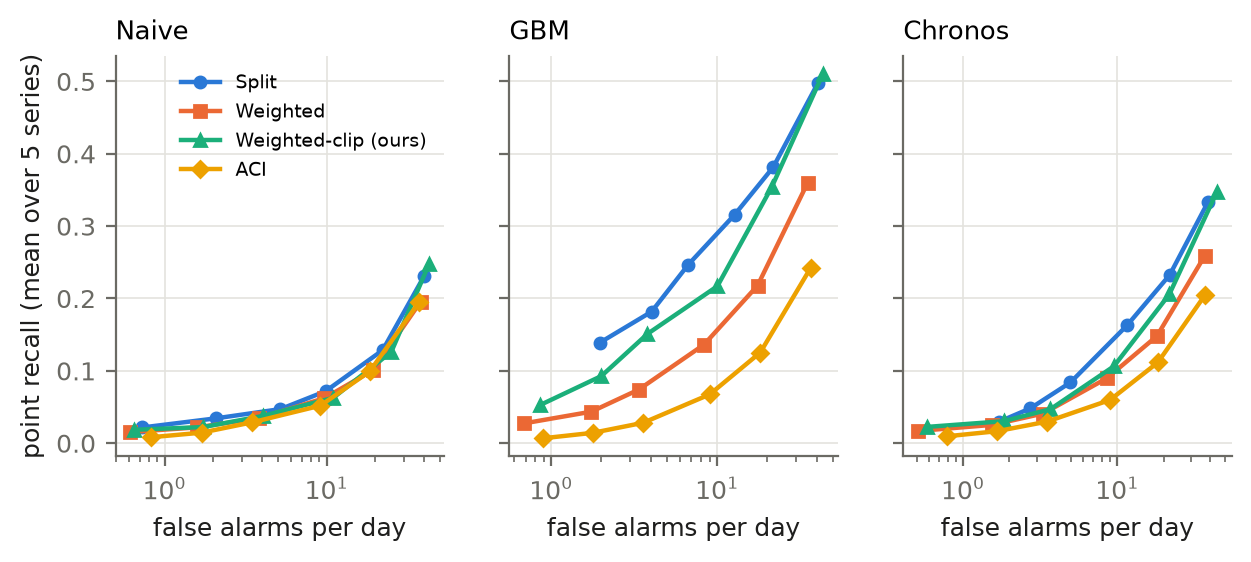
\includegraphics[width=0.76\linewidth]{fig_tradeoff.png}
\caption{Point-level anomaly recall versus false alarms per day as $\alpha$
varies for three representative forecasters. Curves toward the upper-left
are preferable because they detect a larger fraction of anomalous points for
the same operational false-alarm burden. The curves demonstrate that
calibration and detection performance need not rank conformal methods in
the same order.}
\label{fig:tradeoff}
\end{figure}

\begin{figure}[t]
\centering
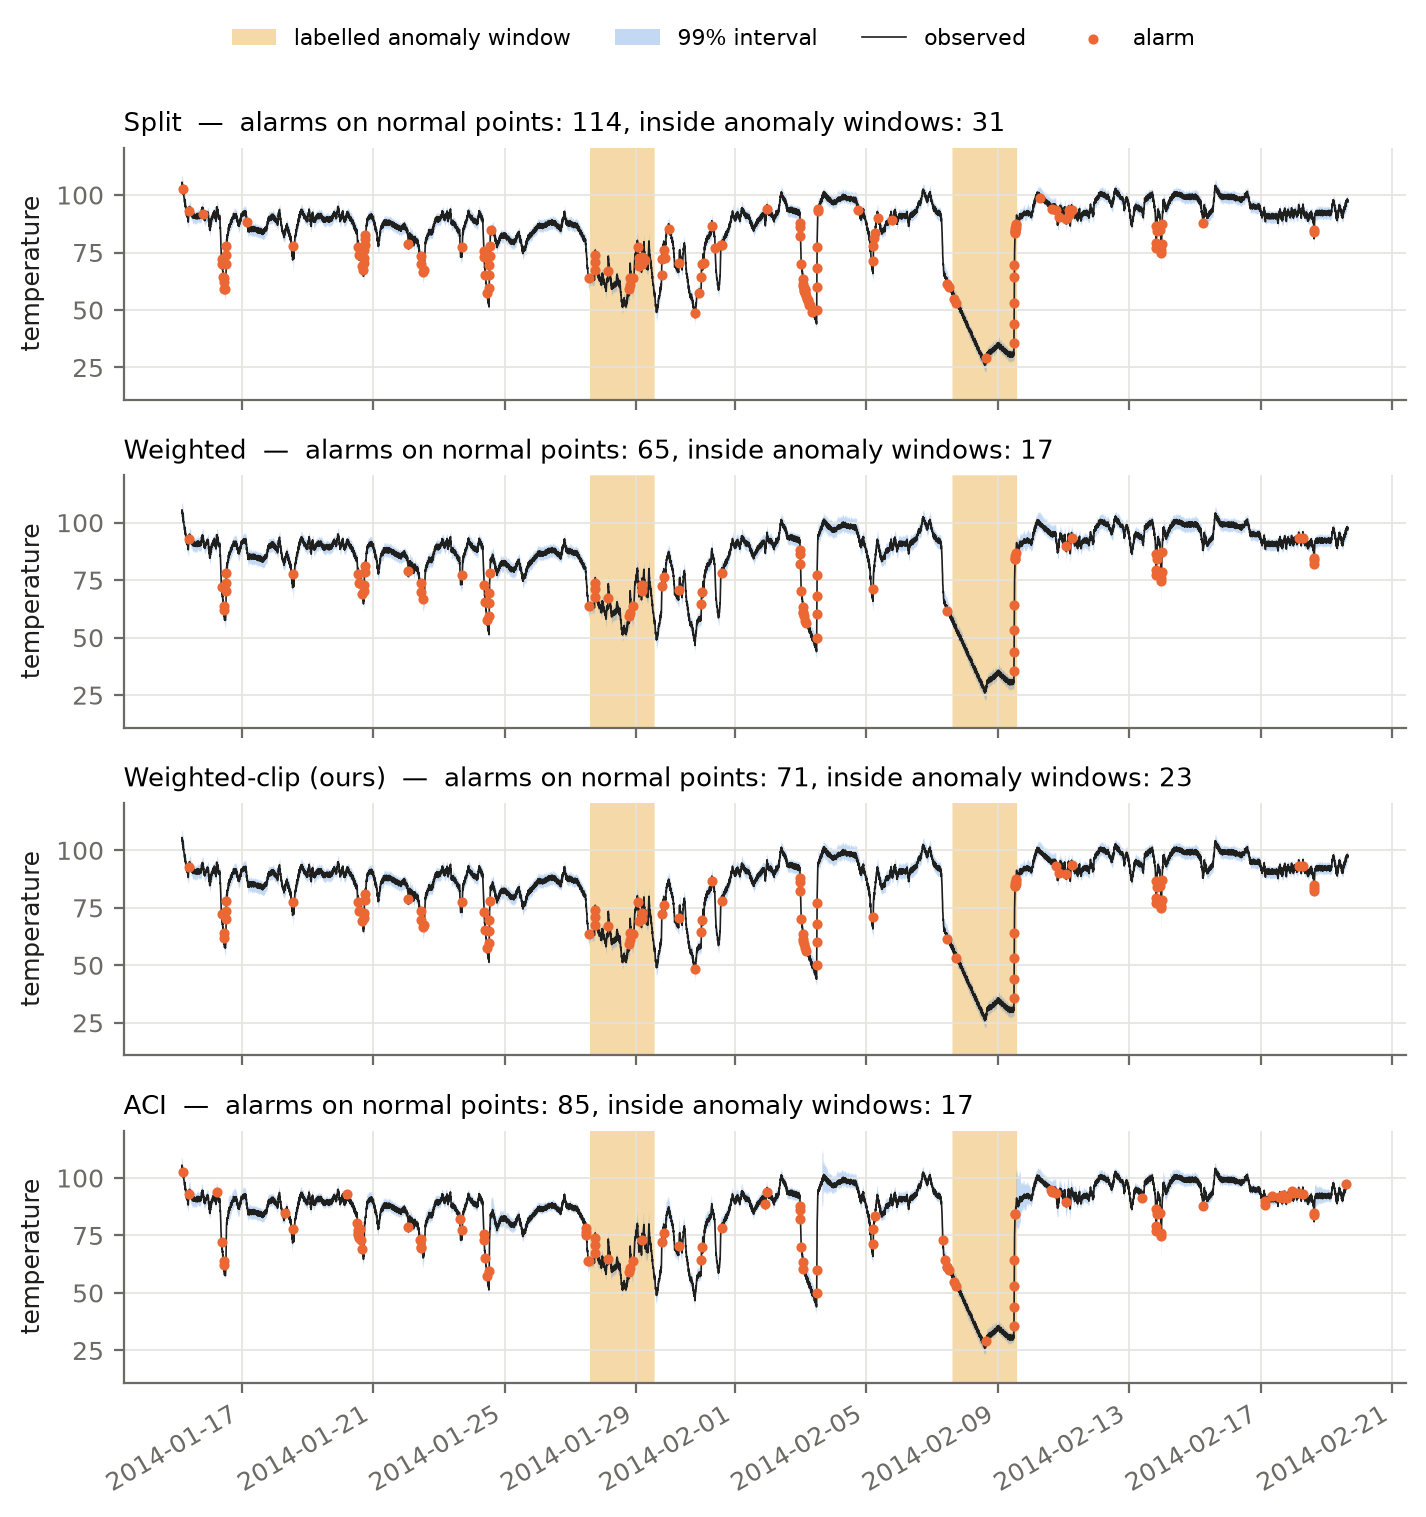
\includegraphics[width=\linewidth,height=0.34\textheight,keepaspectratio]{fig_intervals_machine_temp.png}
\caption{Chronos forecasts on the \texttt{machine\_temp} test segment with
$99\%$ conformal intervals. Shaded regions denote labeled NAB anomaly
windows and alarm markers denote observations outside the conformal
interval. Adaptive procedures widen after repeated exceedances, illustrating
how adaptation to anomalous scores can suppress later alarms within the
same episode.}
\label{fig:intervals}
\end{figure}

\subsection{Episode clipping (our variant)}

Episode clipping was designed specifically to reduce the contamination mechanism identified above. At $\alpha = 0.01$, it increases average F1 from $0.051$ for standard weighted conformal prediction to $0.071$, while normal-point coverage changes only from approximately $99.1\%$ to $98.9\%$. The improvement is particularly pronounced with the gradient-boosting forecaster, for which F1 increases from $0.078$ to $0.151$.

The mechanism is straightforward. Standard weighted conformal prediction assigns high weight to recent anomalous scores. During a persistent failure, these scores rapidly occupy the upper tail of the weighted empirical distribution and increase $q_t$. Episode clipping preserves the first exceedance but limits the magnitude stored for later consecutive exceedances. The detector can therefore adapt to ordinary changes while reducing the ability of a sustained anomalous episode to redefine its own threshold.

Episode clipping is nevertheless not a universally calibrated procedure. At $\alpha = 0.1$, empirical miscoverage rises to approximately $12\%$ rather than the nominal $10\%$. This behavior is consistent with the motivating $\alpha^2$ argument: consecutive false alarms are extremely rare when $\alpha = 0.01$, but become much more common as $\alpha$ increases. We therefore interpret weighted-clip as an empirically useful small-$\alpha$ anomaly-detection modification, not as a method with a proven conformal coverage guarantee.

\subsection{Dependence or shift? (RQ4)}

To investigate why split-conformal coverage deteriorates, we compare its coverage gap with two characteristics of each series--forecaster pair: distribution shift, measured using the KS distance between calibration and test scores, and dependence, summarized by effective calibration size.

The observed association is stronger for shift than for effective sample size, although both correlations are weak. Across the $25$ series--forecaster combinations, the correlation between coverage gap and the shift statistic is approximately $r = +0.28$, whereas the correlation with effective sample size is approximately $r = -0.15$. These values should be interpreted descriptively rather than as statistically conclusive evidence because only $25$ observations contribute to this analysis.

Two series illustrate the distinction. The \texttt{ambient\_temp} series exhibits relatively weak dependence but can have a coverage gap of several percentage points. Its calibration and test periods occur at different portions of the temperature trajectory, making distribution shift a plausible explanation. In contrast, \texttt{nyc\_taxi} exhibits strong temporal dependence through recurring daily and weekly patterns, yet its coverage gap is comparatively small when these patterns remain stable.

This distinction is consistent with the theoretical intuition that dependence and shift affect calibration differently. Temporal dependence reduces the effective amount of independent information available for estimating a quantile, increasing uncertainty or variance in the estimated threshold. Distribution shift changes the score distribution itself, introducing systematic bias when a calibration quantile is applied to a different test distribution. This interpretation is consistent with recent theoretical analyses of predictive inference under temporal dependence \cite{barber2026predictive}.

Therefore, our results do not establish that dependence is harmless. Rather, within this small benchmark, distribution shift appears to be a more visible explanation for large systematic split-conformal coverage gaps than dependence alone.

\begin{figure}[t]
\centering
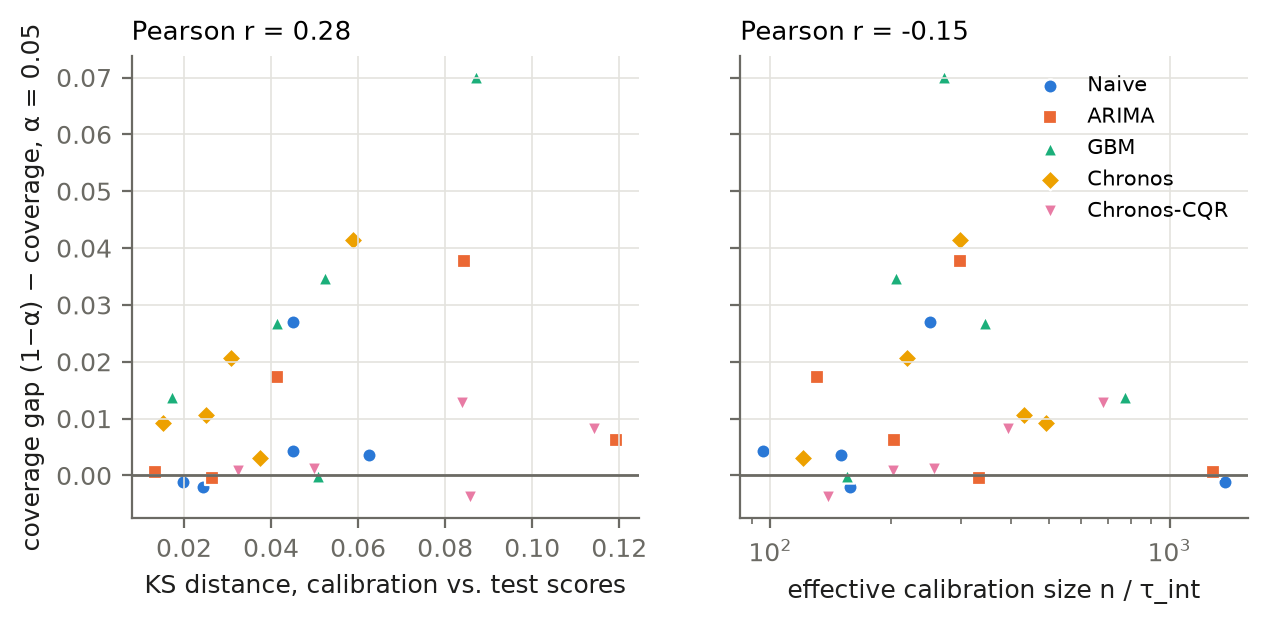
\includegraphics[width=0.76\linewidth]{fig_dependence.png}
\caption{Split-conformal coverage gap at $\alpha = 0.05$ versus distribution
shift measured by the calibration--test KS distance (left) and effective
calibration sample size (right). Each point represents one
series--forecaster combination. The associations are descriptive only
because the analysis contains 25 points.}
\label{fig:dependence}
\end{figure}

\subsection{Does a foundation model help? (RQ3)}

Chronos demonstrates that forecasting accuracy and anomaly-detection performance are distinct objectives. As a zero-shot model, Chronos provides strong normal-period forecasting performance without being fitted to any NAB training series. On \texttt{cpu\_asg}, for example, its normal-point MAE is approximately $0.26$ times that of the naive persistence baseline. It is also competitive on several of the other datasets.

This forecasting advantage does not translate into the highest anomaly-detection F1. With weighted-clip at $\alpha = 0.01$, the gradient-boosting forecaster achieves an average F1 of approximately $0.151$, compared with approximately $0.055$ for the Chronos point forecaster.

Inspection of the predictions suggests a mechanism. Chronos repeatedly receives recent observations as context. Once a failure has persisted long enough to appear throughout that context, the model can follow the changed trajectory. Its predictions then become more accurate \emph{during the anomaly}, reducing the residual $|y_t - \yhat_t|$. A smaller residual makes the observation less anomalous to a residual-based detector.

The gradient-boosting model exhibits almost the opposite behavior. Because tree-based regression generally does not extrapolate beyond values represented by its training leaves, forecasts can become effectively bounded by the range learned from the training data. When the signal moves outside that range during a failure, the model may remain near this ``forecasting floor'' or ceiling and continue producing large residuals. This limitation hurts forecasting under distribution shift but can accidentally benefit anomaly detection.

Consequently, the GBM result should not be interpreted as evidence that it is a universally superior time-series model. Instead, it demonstrates that the best forecasting model is not necessarily the best residual generator for anomaly detection.

This finding mirrors RQ2 at a different level of the pipeline. Adaptation in the \emph{threshold} helps weighted conformal and ACI maintain coverage but can hide persistent anomalies. Adaptation in the \emph{forecaster} helps Chronos follow changing trajectories but can likewise make persistent anomalies appear predictable. In both cases, an anomaly is precisely the behavior to which the detector may not want to adapt too quickly.

\begin{figure}[t]
\centering
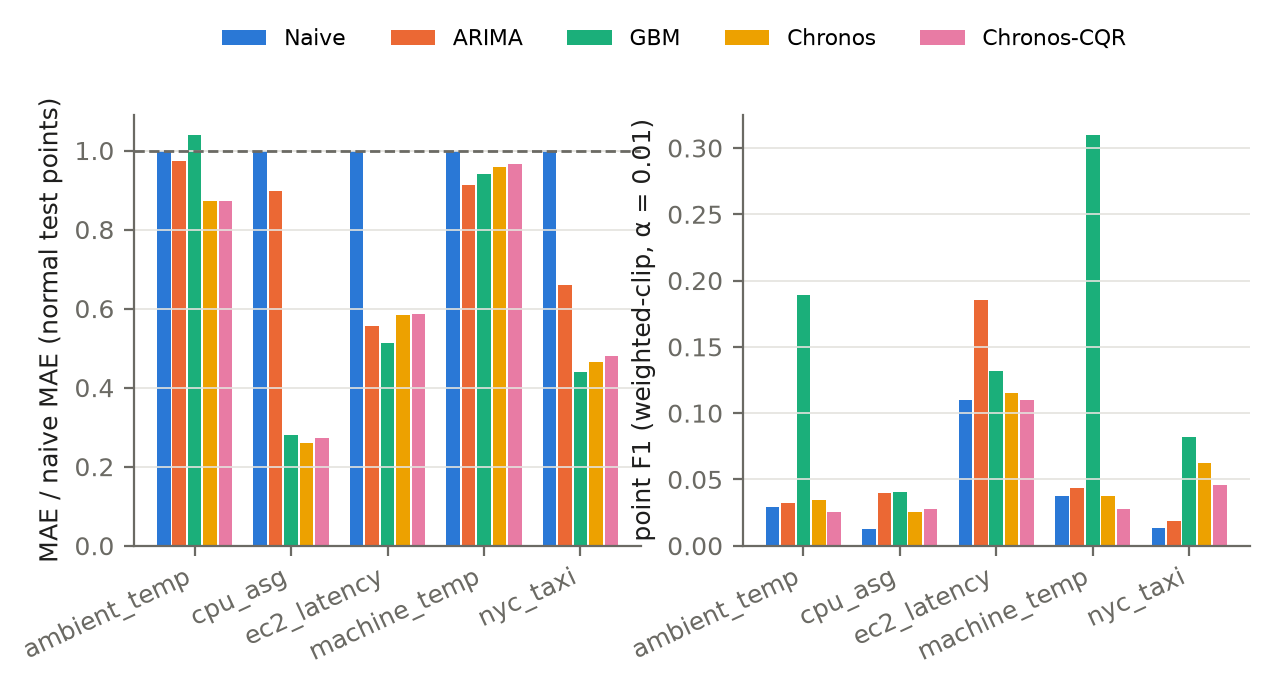
\includegraphics[width=0.76\linewidth]{fig_forecasters.png}
\caption{Forecasting and anomaly-detection performance need not agree.
Left: normal-test MAE relative to the naive persistence forecaster for each
series. Right: point-level detection F1 using weighted-clip at
$\alpha = 0.01$. Chronos can provide highly accurate zero-shot forecasts while
GBM produces higher anomaly-detection F1 in this experiment.}
\label{fig:forecasters}
\end{figure}

\subsection{Sensitivity to hyper-parameters}

The sensitivity experiments further demonstrate that the rate of adaptation is central to the coverage--detection trade-off.

For ACI, $\gamma$ determines how aggressively the effective miscoverage level responds to recent errors. Larger $\gamma$ produces faster correction of miscoverage, but during an anomalous episode it also causes a small number of alarms to widen the prediction interval rapidly. Smaller values of $\gamma$ react less strongly and consequently preserve anomaly recall for longer, at the cost of slower adaptation when genuine distribution shift occurs.

For weighted conformal prediction, $\rho$ controls effective memory. Smaller $\rho$ places greater weight on recent observations and therefore adapts faster. However, the weighted quantile becomes degenerate when the effective history is too short relative to the requested tail probability. For example, at $\rho = 0.99$, $1/(1-\rho) = 100$. At $\alpha = 0.01$, estimating the required upper-tail conformal quantile requires effective support exceeding roughly $1/\alpha$. With only about $100$ effective observations, the conformal construction can place the required quantile at $+\infty$, causing the detector to produce no alarms. This explains the degenerate behavior observed at $\rho = 0.99$.

Thus, $\rho$ and $\gamma$ are not merely numerical tuning parameters. They control how quickly historical information is forgotten and therefore determine how the detector balances responsiveness to distribution shift against resistance to anomalous contamination.

\begin{figure}[t]
\centering
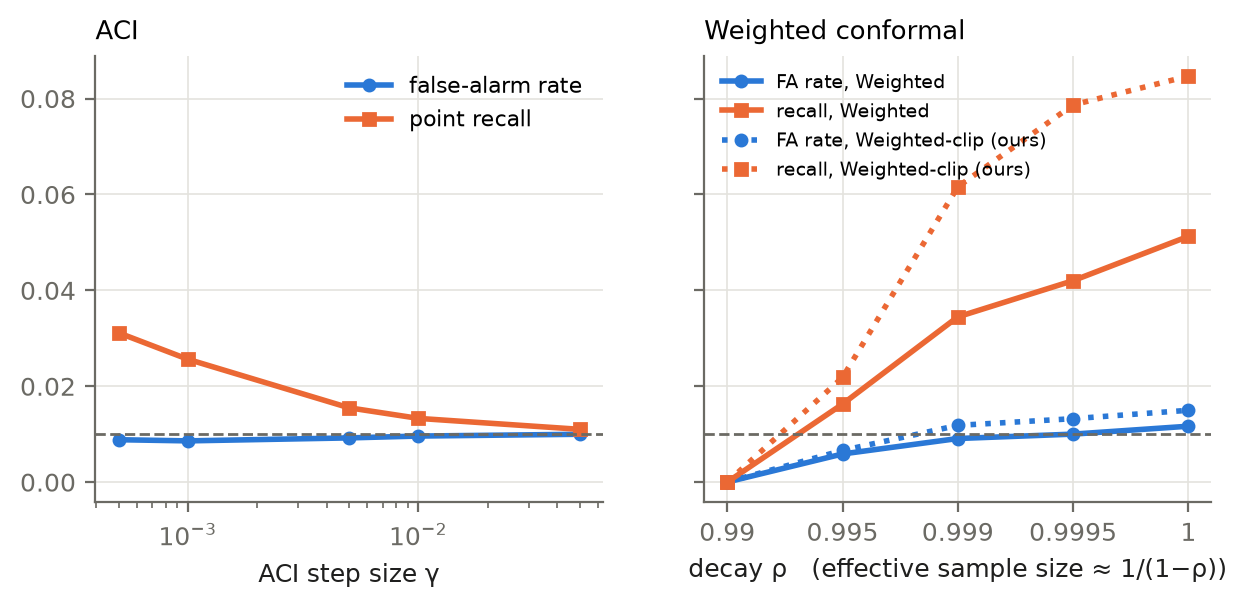
\includegraphics[width=0.76\linewidth]{fig_sensitivity.png}
\caption{Sensitivity to adaptation rate at $\alpha = 0.01$. Left: ACI as the
update step $\gamma$ varies. Right: weighted conformal prediction as the
exponential-decay parameter $\rho$ varies. Results are averaged across the
evaluated series for GBM and Chronos. Aggressive adaptation can improve
responsiveness to shift but reduce anomaly recall or, for insufficient
effective memory, produce a degenerate infinite threshold.}
\label{fig:sensitivity}
\end{figure}

% =====================================================================
\section{Conclusions and Future Work}\label{sec:conclusion}

This project studied reliable time-series anomaly detection through the interaction of forecasting and conformal prediction. Across five NAB time series, five forecasting configurations, and four conformal thresholding strategies, the experiments show that the statistical objective of maintaining predictive coverage and the operational objective of detecting anomalies are related but not equivalent.

First, the finite-sample split-conformal guarantee does not directly carry over to these nonexchangeable time series. At a nominal false-alarm level of $1\%$, split conformal produced approximately $1.56\%$ false alarms, while weighted conformal and ACI remained much closer to the requested level. The i.i.d.\ control experiment indicates that this discrepancy is associated with properties of the time-series data rather than an obvious implementation failure.

Second, the strongest lesson is that adaptation is double-edged. Weighted conformal and ACI protect coverage by responding to recent errors, but during a failure those errors are themselves anomalous. Adapting to them can increase the threshold and suppress later alarms. Episode clipping partially mitigates this effect, improving average F1 from $0.051$ to $0.071$ relative to standard weighted conformal prediction while retaining similar coverage at $\alpha = 0.01$.

The same principle appears at the forecasting level. Chronos provides strong zero-shot forecasting performance, but its ability to follow a changed trajectory can reduce the residuals used to detect persistent failures. In contrast, the less adaptive GBM sometimes produces larger residuals during failures and therefore achieves higher detection F1. Consequently, optimizing forecasting accuracy alone is insufficient when the downstream objective is anomaly detection.

Our exploratory dependence analysis also suggests an important distinction between temporal dependence and distribution shift. Dependence reduces effective calibration information and can increase uncertainty in the estimated conformal threshold, whereas distribution shift can systematically move the test-score distribution away from calibration. In this small experiment, the largest coverage gaps are more consistent with the latter effect, although the sample of $25$ series--forecaster combinations is too small to support a strong causal conclusion.

Several limitations should be emphasized. Only five NAB series were evaluated, and the analysis assumes labeled anomalies can be excluded from the initial calibration partition. NAB's relatively wide anomaly windows also make point-level recall appear low even when most failure windows receive at least one alarm. Only the small Chronos-Bolt model was evaluated, without fine-tuning. The dependence-versus-shift analysis contains only $25$ observations. Finally, episode clipping currently has empirical motivation rather than a formal finite-sample coverage theorem and becomes somewhat anti-conservative at larger $\alpha$.

Overall, the experiments suggest that reliable anomaly detection requires deciding not only \emph{how to adapt}, but also \emph{when adaptation should stop}. A monitoring system should adapt to benign changes in normal behavior without rapidly learning that a genuine failure is the new normal.

\paragraph{Future work.}
\begin{itemize}[leftmargin=*,itemsep=2pt]
  \item Develop a formal coverage or false-alarm bound for episode clipping under exchangeability, mixing, or controlled contamination, and characterize how the probability of consecutive normal exceedances affects that bound.
  \item Extend the detector from point-level residuals to event-level or multi-step conformal scores, and investigate conformal $p$-values with false-discovery-rate control \cite{bates2023testing} for persistent anomaly episodes.
  \item Evaluate larger or fine-tuned time-series foundation models and substantially larger benchmarks, including NASA SMAP/MSL \cite{hundman2018detecting}, to determine whether the observed forecasting--detection trade-off generalizes beyond NAB.
\end{itemize}

% =====================================================================
\bibliographystyle{plainnat}
{\small
\setlength{\bibsep}{2pt plus 1pt}
\bibliography{references}}

\end{document}
